\documentclass[]{scrartcl}
\usepackage{amsmath}
\usepackage{amsfonts}
\usepackage{amssymb}
\usepackage{graphicx}
\usepackage{hyperref}
\usepackage{cleveref}
\usepackage{filecontents}
\usepackage[sort]{natbib}

\title{Theory: Linear elastic active muscle model}
\author{Jean-Paul Pelteret}

\begin{filecontents}{\jobname.bib}
@Article{Kajee2013a,
  author =    {Kajee, Y. and Pelteret, J-P. V. and Reddy, B. D.},
  title =     {The biomechanics of the human tongue},
  journal =   {International Journal for Numerical Methods in Biomedical Engineering},
  year =      {2013},
  volume =    {29},
  number =    {4},
  pages =     {492--514},
  month =     {April},
  doi =       {10.1002/cnm.2531},
  keywords =  {obstructive sleep apnoea ; human tongue ; hill model ; FEM}
}
@Article{Martins1998a,
  Title                    = {A numerical model of passive and active behaviour of skeletal muscles},
  Author                   = {Martins, J. A. C. and Pires, E. B. and Salvado, R. and Dinis, P. B.},
  Journal                  = {Computer Methods in Applied Mechanics and Engineering},
  Year                     = {1998},
  Pages                    = {419--433},
  Volume                   = {151},
  Doi                      = {10.1016/S0045-7825(97)00162-X}
}
@Article{Martins2006a,
  Title                    = {A finite element model of skeletal muscles},
  Author                   = {Martins, J. A. C. and Pato, M. P. M. and Pires, E. B.},
  Journal                  = {Virtual and Physical Prototyping},
  Year                     = {2006},
  Pages                    = {159--170},
  Volume                   = {1},
  Doi                      = {10.1080/17452750601040626}
}
@Article{Pandy1990a,
  Title                    = {An optimal control model for maximum-height human jumping},
  Author                   = {Pandy, M. G. and Zajac, F. E. and Sim, E. and Levine, W. S.},
  Journal                  = {Journal of Biomechanics},
  Year                     = {1990},
  Pages                    = {1185--1198},
  Volume                   = {23},
  Doi                      = {10.1016/0021-9290(90)90376-E}
}
\end{filecontents}

\begin{document}

\maketitle

\begin{abstract}
An introduction to the theory applied to the linear elastic active muscle model of the biceps brachii.
\end{abstract}

\section{Governing equations for quasi-static linear elasticity}
The strong statement of the balance of linear momentum reads
\begin{gather}
\nabla \cdot \boldsymbol{\sigma} + \mathbf{b} 
  = \mathbf{0}
\quad \text{on} \quad \Omega \quad ,
\end{gather}
where $\nabla = \frac{\partial}{\partial x}$ is a differential operator,
$\boldsymbol{\sigma}$ is the Cauchy stress tensor and
$\mathbf{b} = \rho \mathbf{g}$ is the body force density vector.
This is expressed in index notation as
\begin{gather}
\frac{\partial \sigma_{ij}}{\partial x_{j}} + b_{i} 
  = 0
\quad \text{on} \quad \Omega \quad .
\end{gather}
Pre-multiplying the above by test function $\delta \mathbf{v}$ and integrating over the domain $\Omega$ renders
\begin{gather}
- \int\limits_{\Omega} \delta v_{i} \,  \frac{\partial \sigma_{ij}}{\partial x_{j}} \, dv
  = \int\limits_{\Omega} \delta v_{i} \, b_{i} \, dv
\end{gather}
that, by using the product rule for derivatives (i.e. integration by parts), becomes
\begin{gather}
\int\limits_{\Omega} \frac{\partial \delta v_{i}}{\partial x_{j}} \, \sigma_{ij} \, dv
- \int\limits_{\Omega} \frac{\partial}{\partial x_{j}} \left[ \delta v_{i} \, \sigma_{ij} \right] \, dv
  = \int\limits_{\Omega} \delta v_{i} \, b_{i} \, dv
\quad .
\end{gather}
Finally, by applying divergence theorem to the second term in the above, we attain the weak form of the balance of linear momentum
\begin{gather}
\int\limits_{\Omega} \frac{\partial \delta v_{i}}{\partial x_{j}} \, \sigma_{ij} \, dv
  = \int\limits_{\Omega} \delta v_{i} \, b_{i} \, dv
  + \int\limits_{\partial\Omega} \delta v_{i} \, \underbrace{\sigma_{ij} \, n_{j}}_{\bar{t}_{i}} \, da
\quad ,
\label{equ: Weak form of the balance of linear momentum}
\end{gather}
wherein $\mathbf{n}$ represents the outward facing normal on $\partial\Omega$, the boundary of the domain, and $\bar{\mathbf{t}}$ the prescribed traction on the Neumann boundary.

\section{Constitutive law: A linearised Hill three-element active muscle model with surrounding matrix \citep{Kajee2013a}}

The linear constitutive law used to model active muscle tissue is derived by \citep{Kajee2013a} from the nonlinear model developed by \citep{Martins1998a,Martins2006a}.
In the representation given here, we deviate slightly from the notation given in \citep{Kajee2013a} to facilitate its implementation.

\subsubsection*{Embedding of one-dimensional fibre model into three-dimensional space}

We begin by defining the decomposition of the Cauchy stress tensor into a matrix and fibre contribution as
\begin{gather}
\boldsymbol{\sigma}
  = \boldsymbol{\sigma}_{m} + \boldsymbol{\sigma}_{f}
\end{gather}
where $m,f$ respectively denote contributions from the surrounding matrix and muscle fibres.
The isotropic linear constitutive law for the matrix surrounding the muscle fibres is
\begin{gather}
\boldsymbol{\sigma}_{m}
  = \boldsymbol{\mathbb{C}}_{m} : \boldsymbol{\varepsilon}
\end{gather}
where 
$\boldsymbol{\mathbb{C}}_{m}$ is the stiffness tensor for the matrix, and
the small strain tensor
\begin{gather}
\boldsymbol{\varepsilon} 
  = \frac{1}{2} \left[ \nabla \mathbf{u} + \left[ \nabla \mathbf{u} \right]^{T} \right]
\quad .
\end{gather}
The fibre stress and strain are computed by
\begin{gather}
\boldsymbol{\sigma}_{f}
  = T_{f} \mathbf{m} \otimes \mathbf{m}
\quad , \quad
\varepsilon_{f}
  = \left[ \mathbf{m} \otimes \mathbf{m} \right] : \boldsymbol{\varepsilon}
\end{gather}

\subsubsection*{Linearised version of Martin's one-dimensional muscle model}

\Cref{fig: Hill three-element model} shows an analogue for the sarcomere, the smallest building-block of active muscle fibres.
\begin{figure}[!ht]
\centering
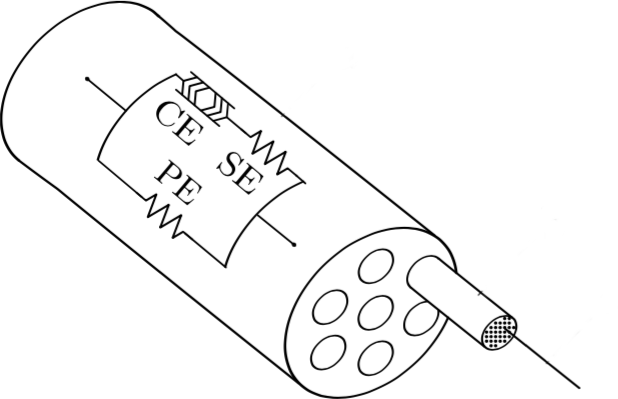
\includegraphics[height=0.23\textheight]{./muscle_fibre-hill_model.png}
\caption{Schematic of the Hill-type muscle fibre \citep{Kajee2013a}.
\label{fig: Hill three-element model}
}
\end{figure}
The distributions of strains and stresses within the various elements of the representative model is determined by their arrangement with respect to one another.
In the linearised (small-strain) version of the Hill three-element model, the decomposition of stress in the fibre as a whole and the one parallel branch are
\begin{gather}
T_{f}
  = T_{p} + T_{s}
\quad\textnormal{and}\quad
T_{c} 
  = T_{s}
\end{gather}
where $T$ is a measure of nominal stress,
and the subscripts $f,p,s,c$ respectively denote the fibre (as a whole), and the parallel, series and contractile element in the Hill model.
Similarly, the decomposition of the (small) strains in the Hill model are
\begin{gather}
\varepsilon_{f}
  = \varepsilon_{p}
  \equiv \varepsilon_{s} + \varepsilon_{c}
\quad .
\end{gather}

The constitutive laws governing the response of each element are as follows:
\begin{gather}
T_{p}
  = T_{0} \,  f_{p}
\quad , \quad
T_{s}
  = T_{0} \,  f_{s}
\quad \textnormal{and} \quad
T_{c}
  = f_{c}^{l} \left( \varepsilon_{c} \right) \, f_{c}^{v} \left( \dot{\varepsilon}_{c} \right) \, \alpha\left( u \left( t \right) \right)
\quad .
\end{gather}
where $T_{0}$ is the nominal stress, a physiological constant which defines to the maximum force of contraction under isometric conditions. 
Here the driver functions for the passive parallel and series elements are
\begin{gather}
f_{p} \left( \varepsilon_{f} \right)
  = \begin{cases}
  m_{p} \varepsilon_{f} \quad &\textnormal{if} \quad \varepsilon_{f} > 0 \\
  0 \quad &\textnormal{otherwise}
  \end{cases}
\\
f_{s} \left( \varepsilon_{s} \right)
  = \begin{cases}
  m_{s} \varepsilon_{s} \equiv m_{s} \left[ \varepsilon_{f} - \varepsilon_{c} \right]  \quad &\textnormal{if} \quad \varepsilon_{s} \equiv \varepsilon_{f} - \varepsilon_{c} > 0 \\
  0 \quad &\textnormal{otherwise}
  \end{cases}
\quad .
\end{gather}
Here the strain relationship between the elements is used to remove $\varepsilon_{s}$ as an unknown.
For the active contractile element, the force-length and force-velocity relationships are approximated as
\begin{gather}
f_{c}^{l} \left( \varepsilon_{c} \right) 
  = \begin{cases}
  1 \quad &\textnormal{if} \quad -0.5 \leq \varepsilon_{c} \leq 0.5 \\
  0 \quad &\textnormal{otherwise}
  \end{cases}
\\
f_{c}^{v} \left( \dot{\varepsilon}_{c} \right)
  = \begin{cases}
  0 &\textnormal{if} \quad \dot{\varepsilon}_{c} < -5 \\
  \frac{1}{5} \dot{\varepsilon}_{c} + 1 &\textnormal{if} \quad  -5 \leq \dot{\varepsilon}_{c} < 3 \\
  1.6 \quad &\textnormal{otherwise}
  \end{cases}
\quad ,
\end{gather}
the latter of which we can write in general as
\begin{gather}
f_{c}^{v} \left( \dot{\varepsilon}_{c} \right)
  = m_{c}^{v} \dot{\varepsilon}_{c} + c_{c}^{v}
\quad .
\end{gather}
Note that alternative linearisations for these terms are possible, and that the rate-dependence of the contractile element makes this model ``visco-elastic''.
The differential equation that defines the muscle activation model \citep{Pandy1990a} is expressed a function of the neural signal $u \left( t \right)$ by
\begin{gather}
\dot{\alpha}\left( u \left( t \right) \right)
  =\frac{1}{\tau_{r}} \left[ 1 - \alpha \right] u + \frac{1}{\tau_{f}} \left[ \alpha_{\min} - \alpha \right] \left[ 1- u \right]
\quad .
\end{gather}
The parameters $\tau_{r}$ and $\tau_{f}$ control the rise and fall of the activation function with respect to the history of the neural signal, and $\alpha_{\min}$ is the minimum activation level (real muscles are never completely inactive; they always retain some degree of tetanisation).

\subsubsection*{Time differentiation}
For all time derivatives we employ a first-order backward Euler scheme.
Therefore the contractile strain rate and rate of change of muscle activation at timestep $n$ are approximated as
\begin{gather}
\dot{\varepsilon}_{c}
  \approx \frac{\varepsilon_{c}^{n} - \varepsilon_{c}^{n-1}}{\Delta t}
\\
\dot{\alpha}
  \approx \frac{{\alpha}^{n} - \alpha^{n-1}}{\Delta t}
\quad .
\end{gather}
Consequently the expression for the force-velocity relationship and activation level can be explicitly stated in terms of the history variables $\varepsilon_{c}^{n-1},\alpha^{n-1}$ and the remaining unknowns $\varepsilon_{c}^{n},\alpha^{n}$.

\subsubsection*{Substitution of fibre constitutive laws into one-dimensional stress relationship}
From the equivalence of $T_{c}$ and $T_{s}$, substituting in all of the salient previously derived expressions and considering $\alpha > 0$, we can extract the explicit expression for $\varepsilon_{c}$ in terms of $\varepsilon_{f}$ by the following steps:
\begin{gather*}
f_{c}^{l} \, f_{c}^{v}  \, \alpha = f_{s} \\
%f_{c}^{l} \, \left[ m_{c}^{v} \dot{\varepsilon}_{c} + c_{c}^{v} \right]  \, \alpha =  m_{s} \left[ \varepsilon_{f} - \varepsilon_{c} \right] \\
\Rightarrow \quad f_{c}^{l} \, \left[ m_{c}^{v} \frac{\varepsilon_{c} - \varepsilon_{c}^{n-1}}{\Delta t} + c_{c}^{v} \right]  \, \alpha =  m_{s} \left[ \varepsilon_{f} - \varepsilon_{c} \right]
\end{gather*}
that, with some further rearrangement, becomes
\begin{align}
\varepsilon_{c}
  &= \underbrace{\left[ f_{c}^{l} m_{c}^{v} \frac{1}{\Delta t} \alpha + m_{s} \right]}_{\beta}\phantom{}^{-1} \left[ m_{s} \varepsilon_{f}  + \underbrace{f_{c}^{l} \alpha \left[ m_{c}^{v} \varepsilon_{c}^{n-1} \frac{1}{\Delta t} - c_{c}^{v} \right]}_{\gamma}\right] \notag\\
  &=  \frac{m_{s}}{\beta} \varepsilon_{f} + \frac{\gamma}{\beta}
\end{align}
Note that $\beta > 0$ under all conditions as $m_{s} > 0$ during contraction.

\subsubsection*{Substitution of constitutive laws into three-dimensional stress relationship}
For the most general case, we can decompose the total Cauchy stress as
\begin{align}
\boldsymbol{\sigma}
  &= \boldsymbol{\mathbb{C}}_{m} : \boldsymbol{\varepsilon} + \boldsymbol{\sigma}_{f} \notag\\
  &= \boldsymbol{\mathbb{C}}_{m} : \boldsymbol{\varepsilon} + T_{f} \mathbf{m} \otimes \mathbf{m} \notag\\
  &= \boldsymbol{\mathbb{C}}_{m} : \boldsymbol{\varepsilon} + T_{0} \left[ m_{p} \varepsilon_{f} + m_{s} \left[ \varepsilon_{f} - \varepsilon_{c} \right] \right] \mathbf{m} \otimes \mathbf{m} \notag\\
  &= \boldsymbol{\mathbb{C}}_{m} : \boldsymbol{\varepsilon} + T_{0} \left[ m_{p} \varepsilon_{f} + m_{s} \left[ \varepsilon_{f} - \left[ \frac{m_{s}}{\beta} \varepsilon_{f} + \frac{\gamma}{\beta} \right] \right] \right] \mathbf{m} \otimes \mathbf{m} \notag\\
  &= \boldsymbol{\mathbb{C}}_{m} : \boldsymbol{\varepsilon} + T_{0} \left[ m_{p} +  m_{s}  - \frac{m_{s}^{2}}{\beta} \right] \varepsilon_{f} \mathbf{m} \otimes \mathbf{m} - \left[ T_{0} m_{s} \frac{\gamma}{\beta} \right] \mathbf{m} \otimes \mathbf{m} \notag\\
  &= \left[ \boldsymbol{\mathbb{C}}_{m} + \underbrace{T_{0} \left[ m_{p} +  m_{s}  - \frac{m_{s}^{2}}{\beta} \right] \mathbf{m} \otimes \mathbf{m} \otimes \mathbf{m} \otimes \mathbf{m} }_{\boldsymbol{\mathbb{C}}_{f}^{\ast}} \right] : \boldsymbol{\varepsilon} \left( \mathbf{u} \right) - \underbrace{\left[ T_{0} m_{s} \frac{\gamma}{\beta} \right] \mathbf{m} \otimes \mathbf{m}}_{\boldsymbol{\sigma}_{f}^{\ast}}
\quad .
\label{equ: Full expansion of constitutive laws}
\end{align}
Note here that the first term on the right hand side ($\left[ \boldsymbol{\mathbb{C}}_{m} + \boldsymbol{\mathbb{C}}_{f}^{\ast} \right] : \boldsymbol{\varepsilon} \left( \mathbf{u} \right)$) is dependent on the solution, and the second term ($\boldsymbol{\sigma}_{f}^{\ast}$) depends only on local history variables.

\section{Finite element discretisation}
Combining \cref{equ: Weak form of the balance of linear momentum,equ: Full expansion of constitutive laws} renders the complete expression of the balance of linear momentum, with accommodation of the muscle fibre model, namely
\begin{gather}
\int\limits_{\Omega} \frac{\partial \delta v_{i}}{\partial x_{j}} \, \left[ \boldsymbol{\mathbb{C}}_{m} + \boldsymbol{\mathbb{C}}_{f}^{\ast} \right]_{ijkl} \varepsilon_{kl} \, dv
  = \int\limits_{\Omega} \delta v_{i} \, b_{i} \, dv
  + \int\limits_{\partial\Omega} \delta v_{i} \, \underbrace{\sigma_{ij} \, n_{j}}_{\bar{t}_{i}} \, da
  - \int\limits_{\Omega} \frac{\partial \delta v_{i}}{\partial x_{j}} \, \left[ \boldsymbol{\sigma}_{f}^{\ast} \right]_{ij} \, dv
\quad ,
\label{equ: Weak form of the balance of linear momentum: Muscle model}
\end{gather}

We discretise the trial solution and test function using finite element shape functions (ansatz)
\begin{gather}
\mathbf{u} \left( \mathbf{x} \right)
  \approx \sum\limits_{I} \boldsymbol{\varPhi}^{I} \left( \mathbf{x} \right) u^{I}
\quad , \quad
\mathbf{v} \left( \mathbf{x} \right)
  \approx \sum\limits_{I} \boldsymbol{\varPhi}^{I} \left( \mathbf{x} \right) v^{I}
\end{gather}
where $\mathbf{N}^{I} \left( \mathbf{x} \right)$ is the (position-dependent) vector-valued finite element shape function corresponding to the $I^{\textnormal{th}}$ degree-of-freedom, and $u^{I}, v^{I}$ are coefficients of the solution and trial function.
In \texttt{deal.II} nomenclature, the shape function is computed from a scalar base shape function and some expansion into higher-dimensional space by
\begin{gather}
\boldsymbol{\varPhi}^{I} \left( \mathbf{x} \right) 
  = N^{I} \left( \mathbf{x} \right) \mathbf{e}_{\textnormal{comp}(I)}
\end{gather}
where $N^{I}$ is a scalar shape function and $\mathbf{e}_{\textnormal{comp}(I)}$ is the basis direction associated with the $I^{\textnormal{th}}$ degree-of-freedom.
Therefore, the $j^{\textnormal{th}}$ local component of shape function $\boldsymbol{\varPhi}^{I} \left( \mathbf{x} \right)$ is given by
\begin{gather}
\left[\boldsymbol{\varPhi}^{I} \left( \mathbf{x} \right)\right]_{j}
  = N^{I} \left( \mathbf{x} \right) \left[ \mathbf{e}_{\textnormal{comp}(I)} \right]_{j}
  = N^{I} \left( \mathbf{x} \right) \delta_{\textnormal{comp}(I) j}
\quad .
\end{gather}
where $\delta_{ij}$ is the Kronecker delta. 
Note that in this instance we use the same ansatz for the test and trial spaces, and the $0 \leq \textnormal{comp}(I), j < \textnormal{spacedim}$.

We now use these shape functions to discretise the weak expression for the balance of linear momentum.
Starting on the right-hand side of \cref{equ: Weak form of the balance of linear momentum: Muscle model}, the body force and traction contributions are computed by
\begin{align}
\int\limits_{\Omega} \delta v_{i} \, b_{i} \, dv
  &= \int\limits_{\Omega} \left[ \sum\limits_{I} \boldsymbol{\varPhi}^{I} \left( \mathbf{x} \right) \delta v^{I} \right]_{i} \, b_{i} \, dv
   = \sum\limits_{I} \delta v^{I} \int\limits_{\Omega} \left[  \boldsymbol{\varPhi}^{I} \left( \mathbf{x} \right) \right]_{i} \, b_{i} \, dv \notag\\
  &= \sum\limits_{I} \delta v^{I} \int\limits_{\Omega} N^{I} \left( \mathbf{x} \right) \delta_{\textnormal{comp}(I) i} \, b_{i} \, dv
   = \sum\limits_{I} \delta v^{I} \int\limits_{\Omega} N^{I} \, b_{\textnormal{comp}(I)} \, dv 
\label{equ: Discretisation: Body force}
\\
\int\limits_{\Omega} \delta v_{i} \, t_{i} \, dv
  &= \sum\limits_{I} \delta v^{I} \int\limits_{\Omega} N^{I} \, t_{\textnormal{comp}(I)} \, dv 
\label{equ: Discretisation: Traction}
\quad .
\end{align}
while the contribution to the right-hand side that arise from the history variables is
\begin{align}
- \int\limits_{\Omega} \frac{\partial}{\partial x_{j}} \left[ \delta v_{i} \right] \, \left[ \boldsymbol{\sigma}_{f}^{\ast} \right]_{ij} \, dv
 &= - \int\limits_{\Omega} \frac{\partial}{\partial x_{j}} \left[ \sum\limits_{I} \boldsymbol{\varPhi}^{I} \left( \mathbf{x} \right) \delta v^{I} \right]_{i} \, \left[ \boldsymbol{\sigma}_{f}^{\ast} \right]_{ij} \, dv \notag\\
 &= - \sum\limits_{I} \delta v^{I} \int\limits_{\Omega} \frac{\partial}{\partial x_{j}} \left[  \boldsymbol{\varPhi}^{I} \left( \mathbf{x} \right)  \right]_{i} \, \left[ \boldsymbol{\sigma}_{f}^{\ast} \right]_{ij} \, dv \notag\\
 &= - \sum\limits_{I} \delta v^{I} \int\limits_{\Omega} \frac{\partial}{\partial x_{j}} \left[  N^{I} \left( \mathbf{x} \right) \delta_{\textnormal{comp}(I) i}  \right] \, \left[ \boldsymbol{\sigma}_{f}^{\ast} \right]_{ij} \, dv \notag\\
 &= - \sum\limits_{I} \delta v^{I} \int\limits_{\Omega} \frac{\partial N^{I} \left( \mathbf{x} \right)}{\partial x_{j}} \, \left[ \boldsymbol{\sigma}_{f}^{\ast} \right]_{\textnormal{comp}(I)j} \, dv 
\label{equ: Discretisation: Stress history}
\quad .
\end{align}
The last component of \cref{equ: Weak form of the balance of linear momentum: Muscle model} that we wish to express in discrete form is the left-hand side of the equation.
Before we do, we observe that using the minor symmetry of the material stiffness tensor we can re-express the contraction of it and the small strain tensor as
\begin{gather}
\boldsymbol{\mathbb{C}} : \boldsymbol{\varepsilon}
  = \boldsymbol{\mathbb{C}} : \frac{1}{2} \left[ \nabla \mathbf{u} + \left[ \nabla \mathbf{u} \right]^{T} \right]
  \equiv \boldsymbol{\mathbb{C}} : \nabla \mathbf{u}
\end{gather}
Therefore, this contribution written in discrete form is
\begin{align}
&\int\limits_{\Omega} \frac{\partial \delta v_{i}}{\partial x_{j}} \, \left[ \boldsymbol{\mathbb{C}}_{m} + \boldsymbol{\mathbb{C}}_{f}^{\ast} \right]_{ijkl} \varepsilon_{kl} \, dv
  \equiv \int\limits_{\Omega} \frac{\partial \delta v_{i}}{\partial x_{j}} \, \mathbb{C}_{ijkl} \, \frac{\partial \delta u_{k}}{\partial x_{l}} \, dv \notag\\
  &\equiv \int\limits_{\Omega} \frac{\partial}{\partial x_{j}} \left[ \sum\limits_{I} \boldsymbol{\varPhi}^{I} \left( \mathbf{x} \right) \delta v^{I} \right]_{i} \, \mathbb{C}_{ijkl} \, \frac{\partial}{\partial x_{l}} \left[ \sum\limits_{J} \boldsymbol{\varPhi}^{J} \left( \mathbf{x} \right) \delta u^{J} \right]_{k} \, dv \notag\\
  &\equiv \sum\limits_{I,J} \delta v^{I} \left[ \int\limits_{\Omega} \frac{\partial}{\partial x_{j}} \left[  \boldsymbol{\varPhi}^{I} \left( \mathbf{x} \right)  \right]_{i} \, \mathbb{C}_{ijkl} \, \frac{\partial}{\partial x_{l}} \left[ \boldsymbol{\varPhi}^{J} \left( \mathbf{x} \right)  \right]_{k} \, dv \right] \delta u^{J} \notag\\
  &\equiv \sum\limits_{I,J} \delta v^{I} \left[ \int\limits_{\Omega} \frac{\partial N^{I} \left( \mathbf{x} \right)}{\partial x_{j}} \delta_{\textnormal{comp}(I) i}  \, \mathbb{C}_{ijkl} \, \frac{\partial  N^{J} \left( \mathbf{x} \right)}{\partial x_{l}} \delta_{\textnormal{comp}(J) k} \, dv \right] \delta u^{J} \notag\\
  &\equiv \sum\limits_{I,J} \delta v^{I} \left[ \int\limits_{\Omega} \frac{\partial N^{I} \left( \mathbf{x} \right)}{\partial x_{j}}  \, \mathbb{C}_{\textnormal{comp}(I) \,j \, \textnormal{comp}(J) \, l} \, \frac{\partial  N^{J} \left( \mathbf{x} \right)}{\partial x_{l}} \, dv \right] \delta u^{J}
\label{equ: Discretisation: Material tangent}
\quad .
\end{align}

\Cref{equ: Discretisation: Body force,equ: Discretisation: Traction,equ: Discretisation: Stress history,equ: Discretisation: Material tangent} are collectively used to develop the system of linear equations that are solved at each time step.

\bibliographystyle{plain}
\bibliography{\jobname} 

\end{document}
